\documentclass{fkpresentation}

% \setcounter{errorcontextlines}{999}
% Information to be included in the title page:
\title{\textmd{The Euler-Lagrange Equation}}
\author{Forest Kobayashi}
\institute{Harvey Mudd College}
\date{April 1st, 2018}

\usepackage{fkmath}
\usepackage{siunitx}
\usepackage{animate}
\usetikzlibrary{external}
\tikzexternalize[prefix=figures/]

\usepackage{subcaption}

\setbeamertemplate{caption}[numbered]

\begin{document}
\frame{\titlepage}
\section{A Motivating Problem}

\begin{frame}{Airlines}
  \begin{figure}[h]
    \centering
    \includegraphics[keepaspectratio, width=.85\linewidth]{figures/airline2.png}
    \caption{Mudd Air; Image adapted from \cite{Airplane}}
  \end{figure}
\end{frame}

\begin{frame}{Airline}
  \begin{figure}[h]
    \centering
    \animategraphics[keepaspectratio,height=6cm,every=3,loop,autoplay]{20}{animations/straight/straight-result-}{0}{128}
    \caption{Flight 1 (UPS9859), Saturday 03/23/2019}
  \end{figure}
\end{frame}

\begin{frame}{Airline, cont.}
  \begin{figure}[h]
    \centering
    \animategraphics[keepaspectratio,height=6cm,every=3,loop,autoplay]{20}{animations/not-straight/not-straight-result-}{0}{115}
    \caption{Flight 2 (FDX50252), Friday 03/22/2019}
  \end{figure}
\end{frame}

% \begin{frame}{Some statistics:}
%   \begin{itemize}
%     \item Total flight distance:
%       \begin{itemize}
%         \item Flight 1: $4551\si{\kilo\meter}$
%         \item Flight 2: $4670\si{\kilo\meter}$
%       \end{itemize}
%     \item Total flight time:
%       \begin{itemize}
%         \item Flight 1: 5h 30min 7s
%         \item Flight 2: 5h 14min 6s
%       \end{itemize}
%     \item Flight 2 went $\sim 100 \si{\kilo\meter}$ further, but arrived $\sim
%       15$ min faster!
%   \end{itemize}
% \end{frame}

\begin{frame}{The difference:}
  \vfill
  \begin{figure}[h]
    \centering
    \animategraphics[keepaspectratio,height=5cm,every=3]{20}{animations/straight/straight-wind-result-}{0}{141}
    \caption{Wind patterns at $70\mrm{hPa}$ during Flight 1}
  \end{figure}
  \vfill
\end{frame}

\begin{frame}{The difference:}
  \vfill
  \begin{figure}[h]
    \centering
    \animategraphics[keepaspectratio,height=5cm,every=3]{20}{animations/not-straight/not-straight-wind-result-}{0}{142}
    \caption{Wind patterns at $70\mrm{hPa}$ during Flight 2}
  \end{figure}
  \vfill
\end{frame}


\begin{frame}{Question:}
  \vfill
  \begin{center}
    \Huge
    How do airlines calculate the best trajectory?
  \end{center}
  \vfill
\end{frame}

\section{Defining the Problem}

\begin{frame}{Big idea: find best path}
  \begin{figure}[h]
    \centering
    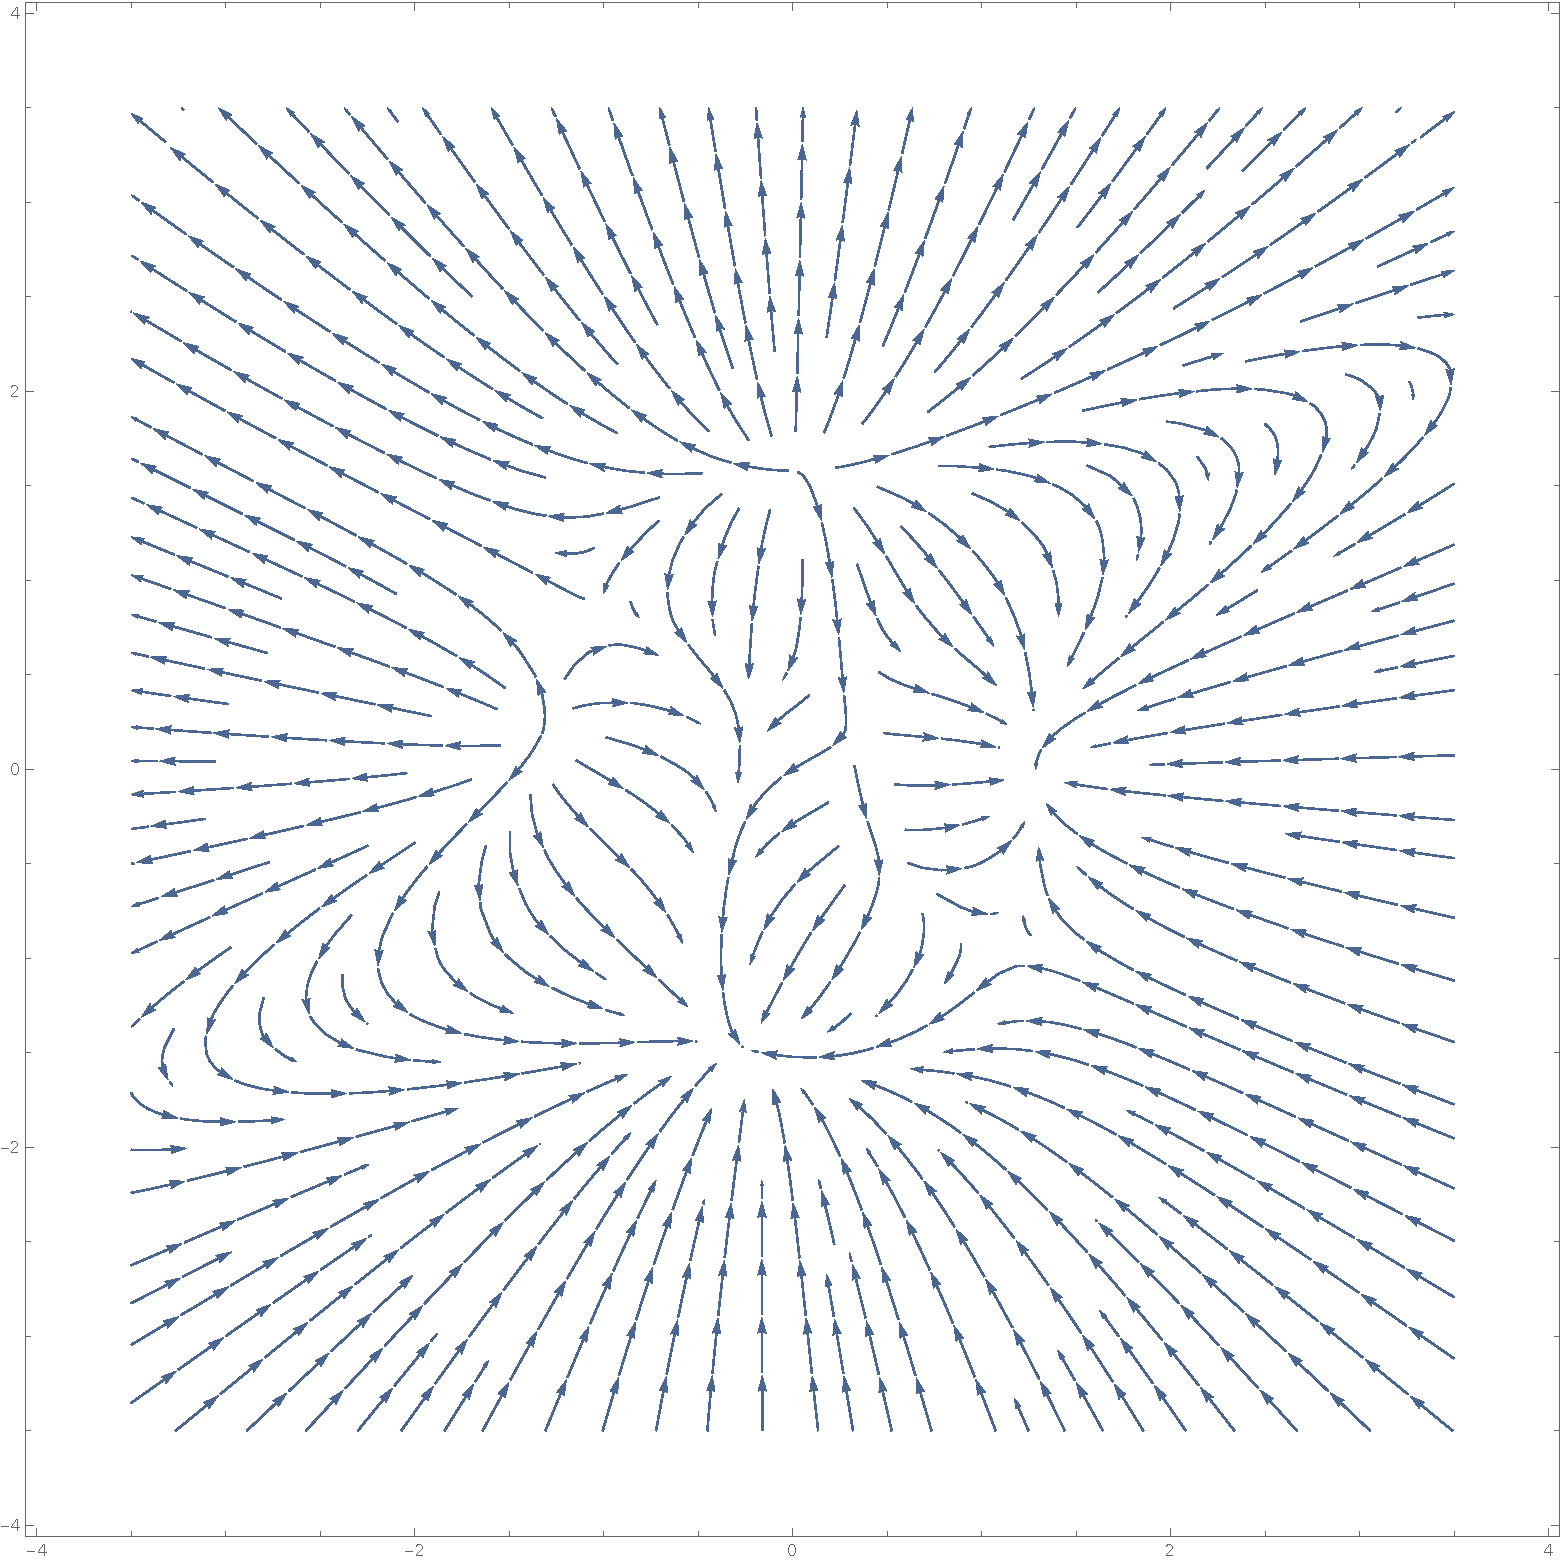
\includegraphics[keepaspectratio,height=5cm]{figures/vector-field.pdf}
    \caption{Drag field}
    \label{fig:wind}
  \end{figure}
\end{frame}

\begin{frame}{Big idea, cont:}
  \begin{figure}[h]
    \vfill
    \centering
    \definecolor{eek}{RGB}{255,255,255}
    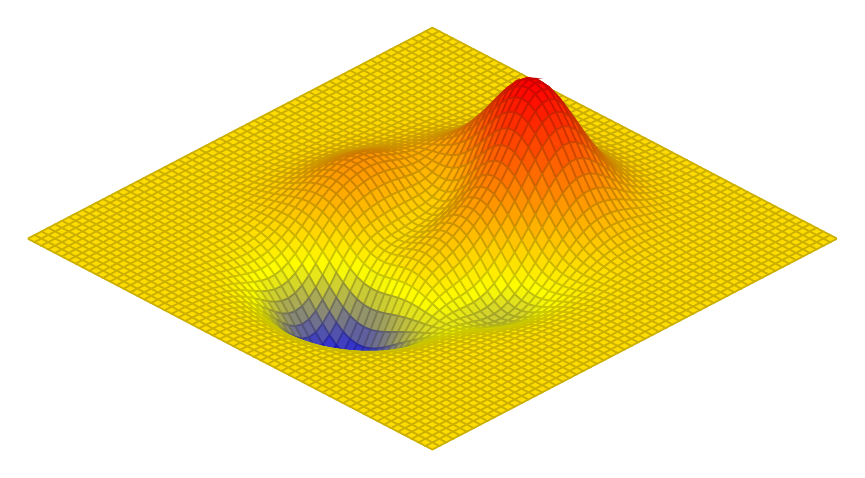
\begin{tikzpicture}[
      scale=1.5,
      declare function = {
        a(\x, \y) = 3*(1-\x)^2 * exp(-(\x^2)-(\y+1)^2);
        b(\x, \y) = -10*(\x/5 - \x^3 + \y^5) * exp(-\x^2 - \y^2);
        c(\x, \y) = -exp(-(\x+1)^2 - \y^2)/3;
        Z(\x, \y) = a(\x,\y) + b(\x,\y) + c(\x,\y);
      }
      ]
      \begin{axis}[
        view={225}{50},
        hide x axis,
        hide y axis,
        hide z axis,
        domain=-3.5:3.5,
        samples=60,
        ]
        \addplot3 [surf] {Z(x,y)};
      \end{axis}
    \end{tikzpicture}
    \vfill
  \end{figure}
\end{frame}

\begin{frame}{Big idea, cont:}
  \begin{figure}[h]
    \vfill
    \centering
    \definecolor{eek}{RGB}{255,255,255}
    \begin{tikzpicture}[
      scale=1.5,
      declare function = {
        a(\x, \y) = 3*(1-\x)^2 * exp(-(\x^2)-(\y+1)^2);
        b(\x, \y) = -10*(\x/5 - \x^3 + \y^5) * exp(-\x^2 - \y^2);
        c(\x, \y) = -exp(-(\x+1)^2 - \y^2)/3;
        Z(\x, \y) = a(\x,\y) + b(\x,\y) + c(\x,\y);
      }
      ]
      \begin{axis}[
        view={225}{50},
        hide x axis,
        hide y axis,
        hide z axis,
        domain=-3.5:3.5,
        samples=60,
        % grid=major,
        ]
        \addplot3 [surf] {Z(x,y)};
        \addplot3 [only marks, mark options={scale=.4}] table[row sep=crcr] {
          x y z \\
          1.5 2 -.558409 \\
          -.5 -1.5 10.2248 \\
        };
        \addplot3 [color=eek, line width=.3mm] table[row sep=crcr] {
          x y z\\
          1.5 2. -0.558409\\
          1.51642 1.94419 -0.563117\\
          1.5281 1.89109 -0.566764\\
          1.5359 1.8402 -0.568777\\
          1.54042 1.79119 -0.568625\\
          1.54169 1.74403 -0.566657\\
          1.53972 1.69873 -0.563314\\
          1.53448 1.6553 -0.559113\\
          1.52618 1.61361 -0.554089\\
          1.51513 1.57349 -0.547923\\
          1.50152 1.53485 -0.540551\\
          1.48554 1.49755 -0.531797\\
          1.46734 1.46152 -0.521699\\
          1.44696 1.42673 -0.51058\\
          1.4246 1.39308 -0.498421\\
          1.40039 1.36049 -0.485341\\
          1.37444 1.32889 -0.471672\\
          1.34694 1.29818 -0.45747\\
          1.31804 1.26827 -0.442899\\
          1.28794 1.23903 -0.427887\\
          1.25679 1.21041 -0.412675\\
          1.22478 1.18227 -0.397133\\
          1.19206 1.15454 -0.381331\\
          1.15877 1.12713 -0.365291\\
          1.12504 1.09997 -0.349063\\
          1.09101 1.073 -0.332668\\
          1.05677 1.04613 -0.316162\\
          1.02244 1.01932 -0.299556\\
          0.9881 0.992514 -0.282893\\
          0.953856 0.965654 -0.266204\\
          0.9198 0.938686 -0.249446\\
          0.886006 0.911568 -0.232734\\
          0.852562 0.88425 -0.216084\\
          0.819556 0.856682 -0.199503\\
          0.787085 0.828809 -0.182967\\
          0.755232 0.800582 -0.166606\\
          0.724107 0.771939 -0.150393\\
          0.69383 0.742811 -0.13433\\
          0.664525 0.713129 -0.118495\\
          0.636327 0.682813 -0.102999\\
          0.609409 0.651766 -0.0878422\\
          0.583954 0.619883 -0.0731155\\
          0.560159 0.587052 -0.0589631\\
          0.538254 0.55314 -0.045439\\
          0.518471 0.518016 -0.0326409\\
          0.501034 0.481552 -0.0206187\\
          0.486106 0.443654 -0.00944393\\
          0.47374 0.404291 0.000850495\\
          0.463844 0.363518 0.010356\\
          0.456166 0.321477 0.0193537\\
          0.450241 0.278434 0.0280568\\
          0.445477 0.234727 0.0366758\\
          0.441231 0.190725 0.0453312\\
          0.436844 0.146804 0.0539149\\
          0.431781 0.103268 0.0624314\\
          0.425606 0.0603679 0.0709817\\
          0.417988 0.0182925 0.0799664\\
          0.408481 -0.0227036 0.0898276\\
          0.396483 -0.0622763 0.10142\\
          0.380887 -0.0997925 0.116149\\
          0.36006 -0.13432 0.137445\\
          0.332543 -0.165025 0.173063\\
          0.300746 -0.193283 0.234018\\
          0.268338 -0.221193 0.324566\\
          0.235187 -0.248678 0.445548\\
          0.20141 -0.275806 0.59699\\
          0.167168 -0.302668 0.777934\\
          0.136 -0.331286 0.977181\\
          0.106559 -0.360891 1.19437\\
          0.0820837 -0.393334 1.41713\\
          0.061576 -0.428043 1.64678\\
          0.0445095 -0.46472 1.88526\\
          0.0319881 -0.503993 2.13105\\
          0.0167515 -0.541715 2.40786\\
          -0.00246576 -0.577162 2.7188\\
          -0.0211968 -0.612888 3.05117\\
          -0.0378337 -0.649809 3.40215\\
          -0.0535971 -0.68723 3.77539\\
          -0.0703844 -0.724066 4.17318\\
          -0.090463 -0.759021 4.59408\\
          -0.117055 -0.790254 5.03122\\
          -0.151035 -0.817266 5.46954\\
          -0.18931 -0.841823 5.89331\\
          -0.233485 -0.863009 6.28331\\
          -0.272369 -0.887218 6.65243\\
          -0.312082 -0.910953 6.9853\\
          -0.350098 -0.935658 7.28763\\
          -0.385309 -0.961966 7.56667\\
          -0.417406 -0.990054 7.82827\\
          -0.447291 -1.0194 8.06996\\
          -0.472559 -1.05139 8.31202\\
          -0.497481 -1.08358 8.52372\\
          -0.518539 -1.11798 8.73285\\
          -0.536287 -1.15426 8.93522\\
          -0.550977 -1.1923 9.12719\\
          -0.56236 -1.23222 9.30809\\
          -0.569452 -1.2746 9.48209\\
          -0.571202 -1.32003 9.65093\\
          -0.565304 -1.36983 9.82094\\
          -0.547243 -1.42658 10.0008\\
          -0.5 -1.5 10.2248\\
        };
      \end{axis}
    \end{tikzpicture}
    \vfill
  \end{figure}
\end{frame}


\begin{frame}{What's essential about this problem?}
  \begin{itemize}
    \item Object of interest: a path $\Qq(t) = (x(t), y(t), z(t))$.
    \item Givens:
      \begin{itemize}
        \item Region we can fly over (Pacific Ocean)
        \item Start/end points: (Honolulu/Anchorage)
        \item Drag: $\mb F_D(t,\, \Qq(t),\, \bm{\dot{q}}(t))$
      \end{itemize}
    \item Goal: find $\Qq(t)$ minimizing \emph{total} travel time.
      % \begin{itemize}
      %   \item Important: total travel time is an ``accumulated cost''
      %   \item Let $\mc L(t,\, \mb x(t),\, \mb{\dot x}(t))$ encode the
      %     ``cost'' of being
      % \end{itemize}
  \end{itemize}
\end{frame}

\begin{frame}{Defining ``Cost''}
  \begin{itemize}
    \item Drag: $\mb F_D(t,\, \Qq(t), \bm{\dot{q}}(t))$
    \item Define ``instantaneous cost'' function:
      \[
        \mc L(t,\, \Qq(t),\, \bm{\dot q}(t))
      \]
    \item Total ``cost'' of trip:
      \[
        C[\Qq] = \int_{t_0}^{t_1} \mc L(t,\, \Qq(t),\, \bm{\dot q}(t))
        \dd t
      \]
    \item What we want: an analogue of the first derivative test
  \end{itemize}
\end{frame}




% \begin{frame}{Translating to the General Case}
%   \begin{columns}
%     \begin{column}{0.5\textwidth}
%       {\large Flight Optimization:}\\[.75em]
%       \begin{itemize}
%         \item Object of interest:
%           \begin{itemize}
%             \item Path $\mb x(t)$
%           \end{itemize}
%         \item Givens:
%           \begin{itemize}
%             \item Domain: region of globe
%             \item End points: HNL, ANC
%             \item Drag: $\mb F(t, \mb x(t),\ \mb v(t))$
%           \end{itemize}
%         \item Goal: find $\mb x(t)$ minimizing travel time
%       \end{itemize}
%     \end{column}\pause
%     \begin{column}{0.5\textwidth}
%       {\large General:}\\[.75em]
%       \begin{itemize}
%         \item Object of interest
%           \begin{itemize}
%             \item A path $\Qq : [t_0, t_f] \to X$
%           \end{itemize}
%         \item Givens:
%           \begin{itemize}
%             \item Domain: some space $X$
%             \item End points: $\Qq(t_0)$, $\Qq(t_f)$
%             \item Cost func: $\mc L(t, \Qq(t), \dot \Qq(t))$
%           \end{itemize}
%         \item
%       \end{itemize}
%     \end{column}
%   \end{columns}
% \end{frame}

% \begin{frame}{Abstracting}
%   \begin{itemize}
%     \item Givens:
%       \begin{itemize}
%         \item A space $X$ we can move through
%         \item A ``cost function''
%       \end{itemize}
%   \end{itemize}
% \end{frame}

% \section{Proof Sketch}

\begin{frame}{Solution: Euler-Lagrange}
  \begin{theorem}[Euler-Lagrange]
    Let $X$ be our space of interest, and let $\Xx_0$, $\Xx_1 \in X$.
    Let $\Qq(t)$ be a path from $\Xx_0$ to $\Xx_1$. Then if $\Qq(t)$
    minimizes the ``total cost function''
    \[
      C[\Qq(t)] = \int_{t_0}^{t_1} \mc L\pn{t, \Qq(t), \dot{\Qq}(t)} \dd
      t,
    \]
    $\Qq(t)$ is a solution to the differential equation
    \[
      \pd{\mc L}{\Qq} - \od{}{t} \pn{\pd{\mc L}{\dot{\Qq}}} = 0.
    \]
  \end{theorem}
\end{frame}

\section{Proof Sketch}
\begin{frame}{Overview (don't sweat the details):}
  \begin{enumerate}
    \item Suppose an optimal $\color{blue} \Qq(t)$ exists.
    \item Take a non-zero path $\color{red} \bm \eta(t)$, with
      ${\color{red}\eta(t_0)} = 0 = {\color{red}\eta(t_f)}$.
    \item For all ${\color{red}\alpha} \neq 0$, the path $\bm{q'}(t) =
      {\color{blue} \Qq(t)} + {\color{red} \alpha \cdot \bm{\eta}(t)}$
      is not optimal.
    \item Thus, $C[\Qq'(t)]$ is minimized when $\color{red}\alpha =
      0$.
    \item Applying the first derivative test in $\color{red} \alpha$,
      we can show
      \[
        \od{C}{{\color{red}\alpha}} \bigg\vert_{{\color{red}\alpha}=0}
        = \int_{t_0}^{t_1} \bk{\pd{\mc L}{\color{blue} \Qq} -
          \od{}{t}\pn{\pd{\mc L}{\color{blue} \bm{\dot q}}}}
        {\color{red}\eta(t)} \dd t = 0
      \]
      and the result follows.
  \end{enumerate}
\end{frame}
\begin{frame}{Suppose an optimal $\color{blue}\Qq(t)$ exists:}
  \begin{figure}[h]
    \centering
    \begin{tikzpicture}[scale=1.15,
      declare function = {
        epsilon(\x) = .06;
        fopt(\x) = -1.7 + \x * (3.31667 + (-0.9 + 0.0833333 * \x) * \x);
        eta(\x) = epsilon(0)*((.5+2*sin(2*\x-2) * exp(2-1 * \x)) * (\x - 5.5) * (\x - 1.5))^2;
        fprime(\x) = fopt(\x) + eta(\x);
      }
      ]
      \pgfmathsetmacro{\xmin}{-.2};
      \pgfmathsetmacro{\ymin}{-.2};
      \pgfmathsetmacro{\xmax}{6};
      \pgfmathsetmacro{\ymax}{4};

      \pgfmathsetmacro{\qs}{1.56875};
      \pgfmathsetmacro{\qf}{3.18126};

      \pgfmathsetmacro{\extraforaxes}{.2};

      \pgfmathsetmacro{\epsilon}{.06};

      \draw[->] (\xmin,0) -- (\xmax+\extraforaxes, 0) node[below] {$x$};
      \draw[->] (0,\ymin) -- (0, \ymax+\extraforaxes) node[left] {$y$};

      % Optimal y
      \draw[domain=1.5:5.5, smooth, variable=\x, blue] plot ({\x-.5}, {fopt(\x)});

      \node[below right] at (4.25, 2.75) {$\color{blue} \bm{q}(t)$};

      \node[
      circle,
      draw=black,
      fill=white,
      inner sep=0pt,
      minimum size=5pt
      ] (y0) at (1, 1.56875) {};

      \node[
      circle,
      draw=black,
      fill=white,
      inner sep=0pt,
      minimum size=5pt
      ] (y1) at (5, 3.18126) {};

      \node[below,yshift=-4pt] (t0) at (1, 0) {$t_0$};
      \node[below,yshift=-4pt] (t1) at (5, 0) {$t_1$};
      \draw[dotted] (y0) -- (1,0);
      \draw[dotted] (y1) -- (5,0);
      \draw (1,.08) -- (1,-.08);
      \draw (5,.08) -- (5,-.08);

      \node[left,xshift=-4pt] (q0) at (0,\qs) {$\color{blue}\Qq(t_0)$};
      \node[left,xshift=-4pt] (qf) at (0,\qf) {$\color{blue}\Qq(t_f)$};
      \draw[dotted] (0,\qs) -- (y0);
      \draw[dotted] (0,\qf) -- (y1);
      \draw (-.08,\qs) -- (.08,\qs);
      \draw (-.08,\qf) -- (.08,\qf);
    \end{tikzpicture}
    \caption{Optimal $\color{blue} \Qq(t)$}
  \end{figure}
\end{frame}

\begin{frame}{For some $\color{red} \bm{\eta}(t)$, add $\color{red}\alpha \cdot \bm{\eta}(t)$:}
  \begin{figure}[h]
    \centering
    \begin{tikzpicture}[scale=1.15,
      declare function = {
        epsilon(\x) = .06;
        fopt(\x) = -1.7 + \x * (3.31667 + (-0.9 + 0.0833333 * \x) * \x);
        eta(\x) = epsilon(0)*((.5+2*sin(2*\x-2) * exp(2-1 * \x)) * (\x - 5.5) * (\x - 1.5))^2;
        fprime(\x) = fopt(\x) + eta(\x);
      }
      ]
      \pgfmathsetmacro{\xmin}{-.2};
      \pgfmathsetmacro{\ymin}{-.2};
      \pgfmathsetmacro{\xmax}{6};
      \pgfmathsetmacro{\ymax}{4};

      \pgfmathsetmacro{\qs}{1.56875};
      \pgfmathsetmacro{\qf}{3.18126};

      \pgfmathsetmacro{\extraforaxes}{.2};

      \pgfmathsetmacro{\epsilon}{.06};

      \draw[->] (\xmin,0) -- (\xmax+\extraforaxes, 0) node[below] {$x$};
      \draw[->] (0,\ymin) -- (0, \ymax+\extraforaxes) node[left] {$y$};

      % Optimal y
      \draw[domain=1.5:5.5, smooth, variable=\x, blue] plot ({\x-.5}, {fopt(\x)});

      % Perturbation
      \draw[domain=1.5:5.5, smooth, variable=\x, densely dotted, thick] plot ({\x-.5}, {fprime(\x)});
      \draw[domain=1.5:5.5, smooth, variable=\x, red] plot ({\x-.5}, {eta(\x)});

      \node[
      circle,
      draw=black,
      fill=white,
      inner sep=0pt,
      minimum size=5pt
      ] (y0) at (1, 1.56875) {};

      \node[
      circle,
      draw=black,
      fill=white,
      inner sep=0pt,
      minimum size=5pt
      ] (y1) at (5, 3.18126) {};

      \node[above] at (3,.3) {$\color{red} \alpha \cdot \bm{\eta}(t)$};
      \node[below right] at (4.25, 2.75) {$\color{blue} \bm{q}(t)$};
      \node[above left] at (2.6,2.68) {$\bm{q'}(t)$};


      \node[below,yshift=-4pt] (t0) at (1, 0) {$t_0$};
      \node[below,yshift=-4pt] (t1) at (5, 0) {$t_1$};
      \draw[dotted] (y0) -- (1,0);
      \draw[dotted] (y1) -- (5,0);
      \draw (1,.08) -- (1,-.08);
      \draw (5,.08) -- (5,-.08);

      \node[left,xshift=-4pt] (q0) at (0,\qs) {$\color{blue}\Qq(t_0)$};
      \node[left,xshift=-4pt] (qf) at (0,\qf) {$\color{blue}\Qq(t_f)$};
      \draw[dotted] (0,\qs) -- (y0);
      \draw[dotted] (0,\qf) -- (y1);
      \draw (-.08,\qs) -- (.08,\qs);
      \draw (-.08,\qf) -- (.08,\qf);

    \end{tikzpicture}
    \caption{Add a small perturbation ${\color{red}\alpha \cdot \bm \eta(t)}$}
  \end{figure}
\end{frame}

\begin{frame}{$\Qq'(t)$ for various values of $\color{red} \alpha$:}
  \begin{figure}[h]
    \centering
    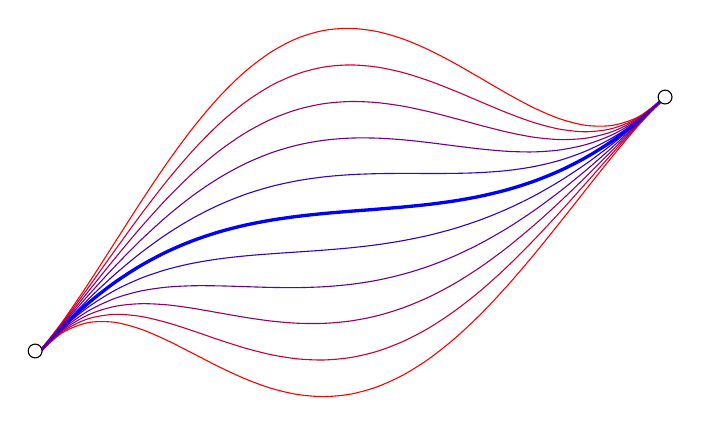
\begin{tikzpicture}[%
      scale=2, %
      declare function = {
        fopt(\x) = -1.7 + \x * (3.31667 + (-0.9 + 0.0833333 * \x) * \x);
        eta(\x,\alpha) = \alpha*((.5+2*sin(2*\x-2) * exp(2-1 * \x)) * (\x - 5.5) * (\x - 1.5))^2;
        fprime(\x,\alpha) = fopt(\x) + eta(\x,\alpha);
      }
      ]
      \pgfmathsetmacro{\xmin}{-.2};
      \pgfmathsetmacro{\ymin}{-.2};
      \pgfmathsetmacro{\xmax}{6};
      \pgfmathsetmacro{\ymax}{4};

      \pgfmathsetmacro{\qs}{1.56875};
      \pgfmathsetmacro{\qf}{3.18126};

      \pgfmathsetmacro{\extraforaxes}{.2};

      \pgfmathsetmacro{\epsilon}{.06};

      % Optimal y
      \draw[domain=1.5:5.5, smooth, variable=\x, blue, very thick] plot ({\x-.5}, {fopt(\x)});

      % Perturbation
      \foreach \alpha/\thecolor in {%
        0.25/red,%
        0.20/red!80!blue,%
        0.15/red!60!blue,%
        0.10/red!40!blue,%
        0.05/red!20!blue%
      }{
        \draw[domain=1.5:5.5, smooth, variable=\x,\thecolor] plot ({\x-.5}, {fprime(\x,\alpha)});
        \draw[domain=1.5:5.5, smooth, variable=\x,\thecolor] plot ({\x-.5}, {fprime(\x,-1*\alpha)});
      }
      \node[
      circle,
      draw=black,
      fill=white,
      inner sep=0pt,
      minimum size=5pt
      ] (y0) at (1, 1.56875) {};

      \node[
      circle,
      draw=black,
      fill=white,
      inner sep=0pt,
      minimum size=5pt
      ] (y1) at (5, 3.18126) {};

    \end{tikzpicture}
    \caption{$\bm{q'}(t)$ for various values of $\color{red}\alpha$}
  \end{figure}
  \vfill
\end{frame}

\begin{frame}{Turn $C$ into optimizing a 1-D function:}
  \begin{itemize}
    \item Consider $C[\bm{q'}(t)]$ as a function of just $\color{red}
      \alpha$:
      \[
        C'({\color{red}\alpha})
        = C\bk{{\color{blue}\bm{q}(t)} + {\color{red}\alpha \cdot
            \bm{\eta}(t)}}.
      \]
      This is just a map from $\RR\to \RR$!
    \item Note that $C'({\color{red} 0}) = C[{\color{blue} \Qq(t)}]$,
      so
      \[
        0 = \od{C'({\color{red} \alpha})}{\color{red}\alpha}
        \bigg\vert_{{\color{red}\alpha} = 0}
      \]
    \item Repeated application of the chain rule and integration by
      parts yields the desired result!
  \end{itemize}
\end{frame}



\section{Other examples}

\begin{frame}{Examples}
  \begin{itemize}
    \item Lagrangian Mechanics
    \item Brachistochrone problem
    \item Optimal control
    \item Geodesics
    \item Minimal surfaces of revolution
  \end{itemize}
\end{frame}

\begin{frame}{Brachistochrone}
  \vfill
  \begin{figure}[h]
    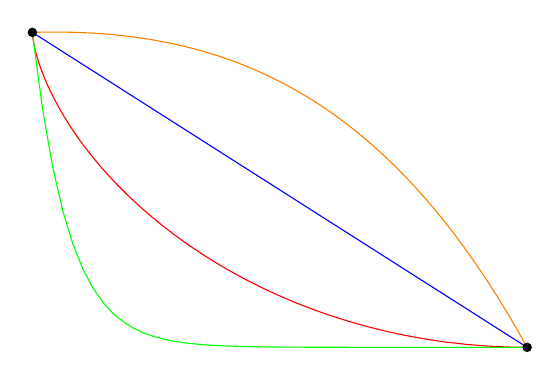
\begin{tikzpicture}[scale=2]
      \def\r{1} % radius
      \def\c{1.4} % center
      \coordinate (O) at (0,0);
      \coordinate (A) at (0,2*\r);
      \coordinate (B) at (pi, 0);

      % Cycloid
      \draw[red,domain=0:pi,samples=50] plot ({\x - sin(\x r)},{\r+cos(\x r)});

      % Straight line
      \draw[blue] (A) -- (B);

      % The other two
      \draw[green, domain=0:pi, samples=50] plot ({\x}, {(-2/pi)*(\x-pi)*exp(-4*\x)});
      \draw[orange, domain=0:pi, samples=50] plot ({\x}, {(-2/pi)*(\x-pi)*exp(\x/3)});

      % Release point
      \draw[fill=black] (A) circle (.75pt);

      % End point
      \draw[fill=black] (B) circle (.75pt);

    \end{tikzpicture}
  \end{figure}
  \vfill
\end{frame}

\section{Bibliography}
\begin{frame}
  \frametitle{References}
  \bibliographystyle{alpha}
  % \bibliographystyle{IEEE}
  \bibliography{talk5.bib}
\end{frame}

\end{document}


%%% Local Variables:
%%% TeX-master: t
%%% TeX-engine: default-shell-escape
%%% TeX-command-extra-option: -pdf
%%% End: